\documentclass[a4paper]{article}
\usepackage[12pt]{extsizes}
\usepackage[utf8]{inputenc}
\usepackage[russian]{babel}
\usepackage{setspace}
\usepackage{amsmath}
\usepackage[left=10mm, top=15mm, right=10mm, bottom=15mm, nohead, footskip=10mm]{geometry} 
\usepackage{wrapfig}
\usepackage[pdftex]{graphicx}
\usepackage{indentfirst}
\graphicspath{{pictures/}}
\DeclareGraphicsExtensions{.eps,.pdf,.png,.jpg}
\begin{document}
\setcounter{page}{0} 
\begin{titlepage}
\begin{center}
\largel{\textbf{МОСКОВСКИЙ ГОСУДАРСТВЕННЫЙ УНИВЕРСИТЕТ\\ИМЕНИ М.В. ЛОМОНОСОВА}}\\
\hfill\break
\normalsize{ФИЗИЧЕСКИЙ ФАКУЛЬТЕТ}\\
 \hfill\break
\normalsize{ГОСУДАРСТВЕННЫЙ АСТРОНОМИЧЕСКИЙ ИНСТИТУТ ИМЕНИ П.К. ШТЕРНБЕРГА}\\
\hfill\break
\hfill\break
\hfill\break
\hfill\break
\hfill\break
\hfill\break
\hfill\break
\hfill\break
\largel{\textbf{ОПРЕДЕЛЕНИЕ ЭФФЕКТИВНОСТИ ИНФРАКТРАСНОЙ КАМЕРЫ\\ПРИ РАБОТЕ В СПЕКТРОСКОПИЧЕСКОМ РЕЖИМЕ}\\
\hfill\break
\normalsize{(Н.А. МИТИЧКИН, И.А. ОРЛОВ)}\\
\hfill\break
\normalsize{РУКОВОДИТЕЛЬ: А.М. ТАТАРНИКОВ}\\
\end{center}
\hfill\break
\hfill\break
\hfill\break
\hfill\break
\hfill\break
\hfill\break
\hfill\break
\hfill\break
\hfill\break
\hfill\break
\hfill\break
\hfill\break
\hfill\break
\hfill\break
\hfill\break
\hfill\break 
\hfill\break
\hfill\break
\hfill\break
\hfill\break
\hfill\break
\hfill\break
\hfill\break
\hfill\break
\hfill\break
\hfill\break
\hfill\break
\begin{center}
Кавказская горная обсерватория ГАИШ МГУ имени М.В. Ломоносова, июль 2018 г.
\end{center}
\thispagestyle{empty}
\end{titlepage}
\newpage
\tableofcontents
\newpage
\section{Введение}
\begin{wrapfigure}[12]{r}{0.40\linewidth} 
\vspace{-4ex}
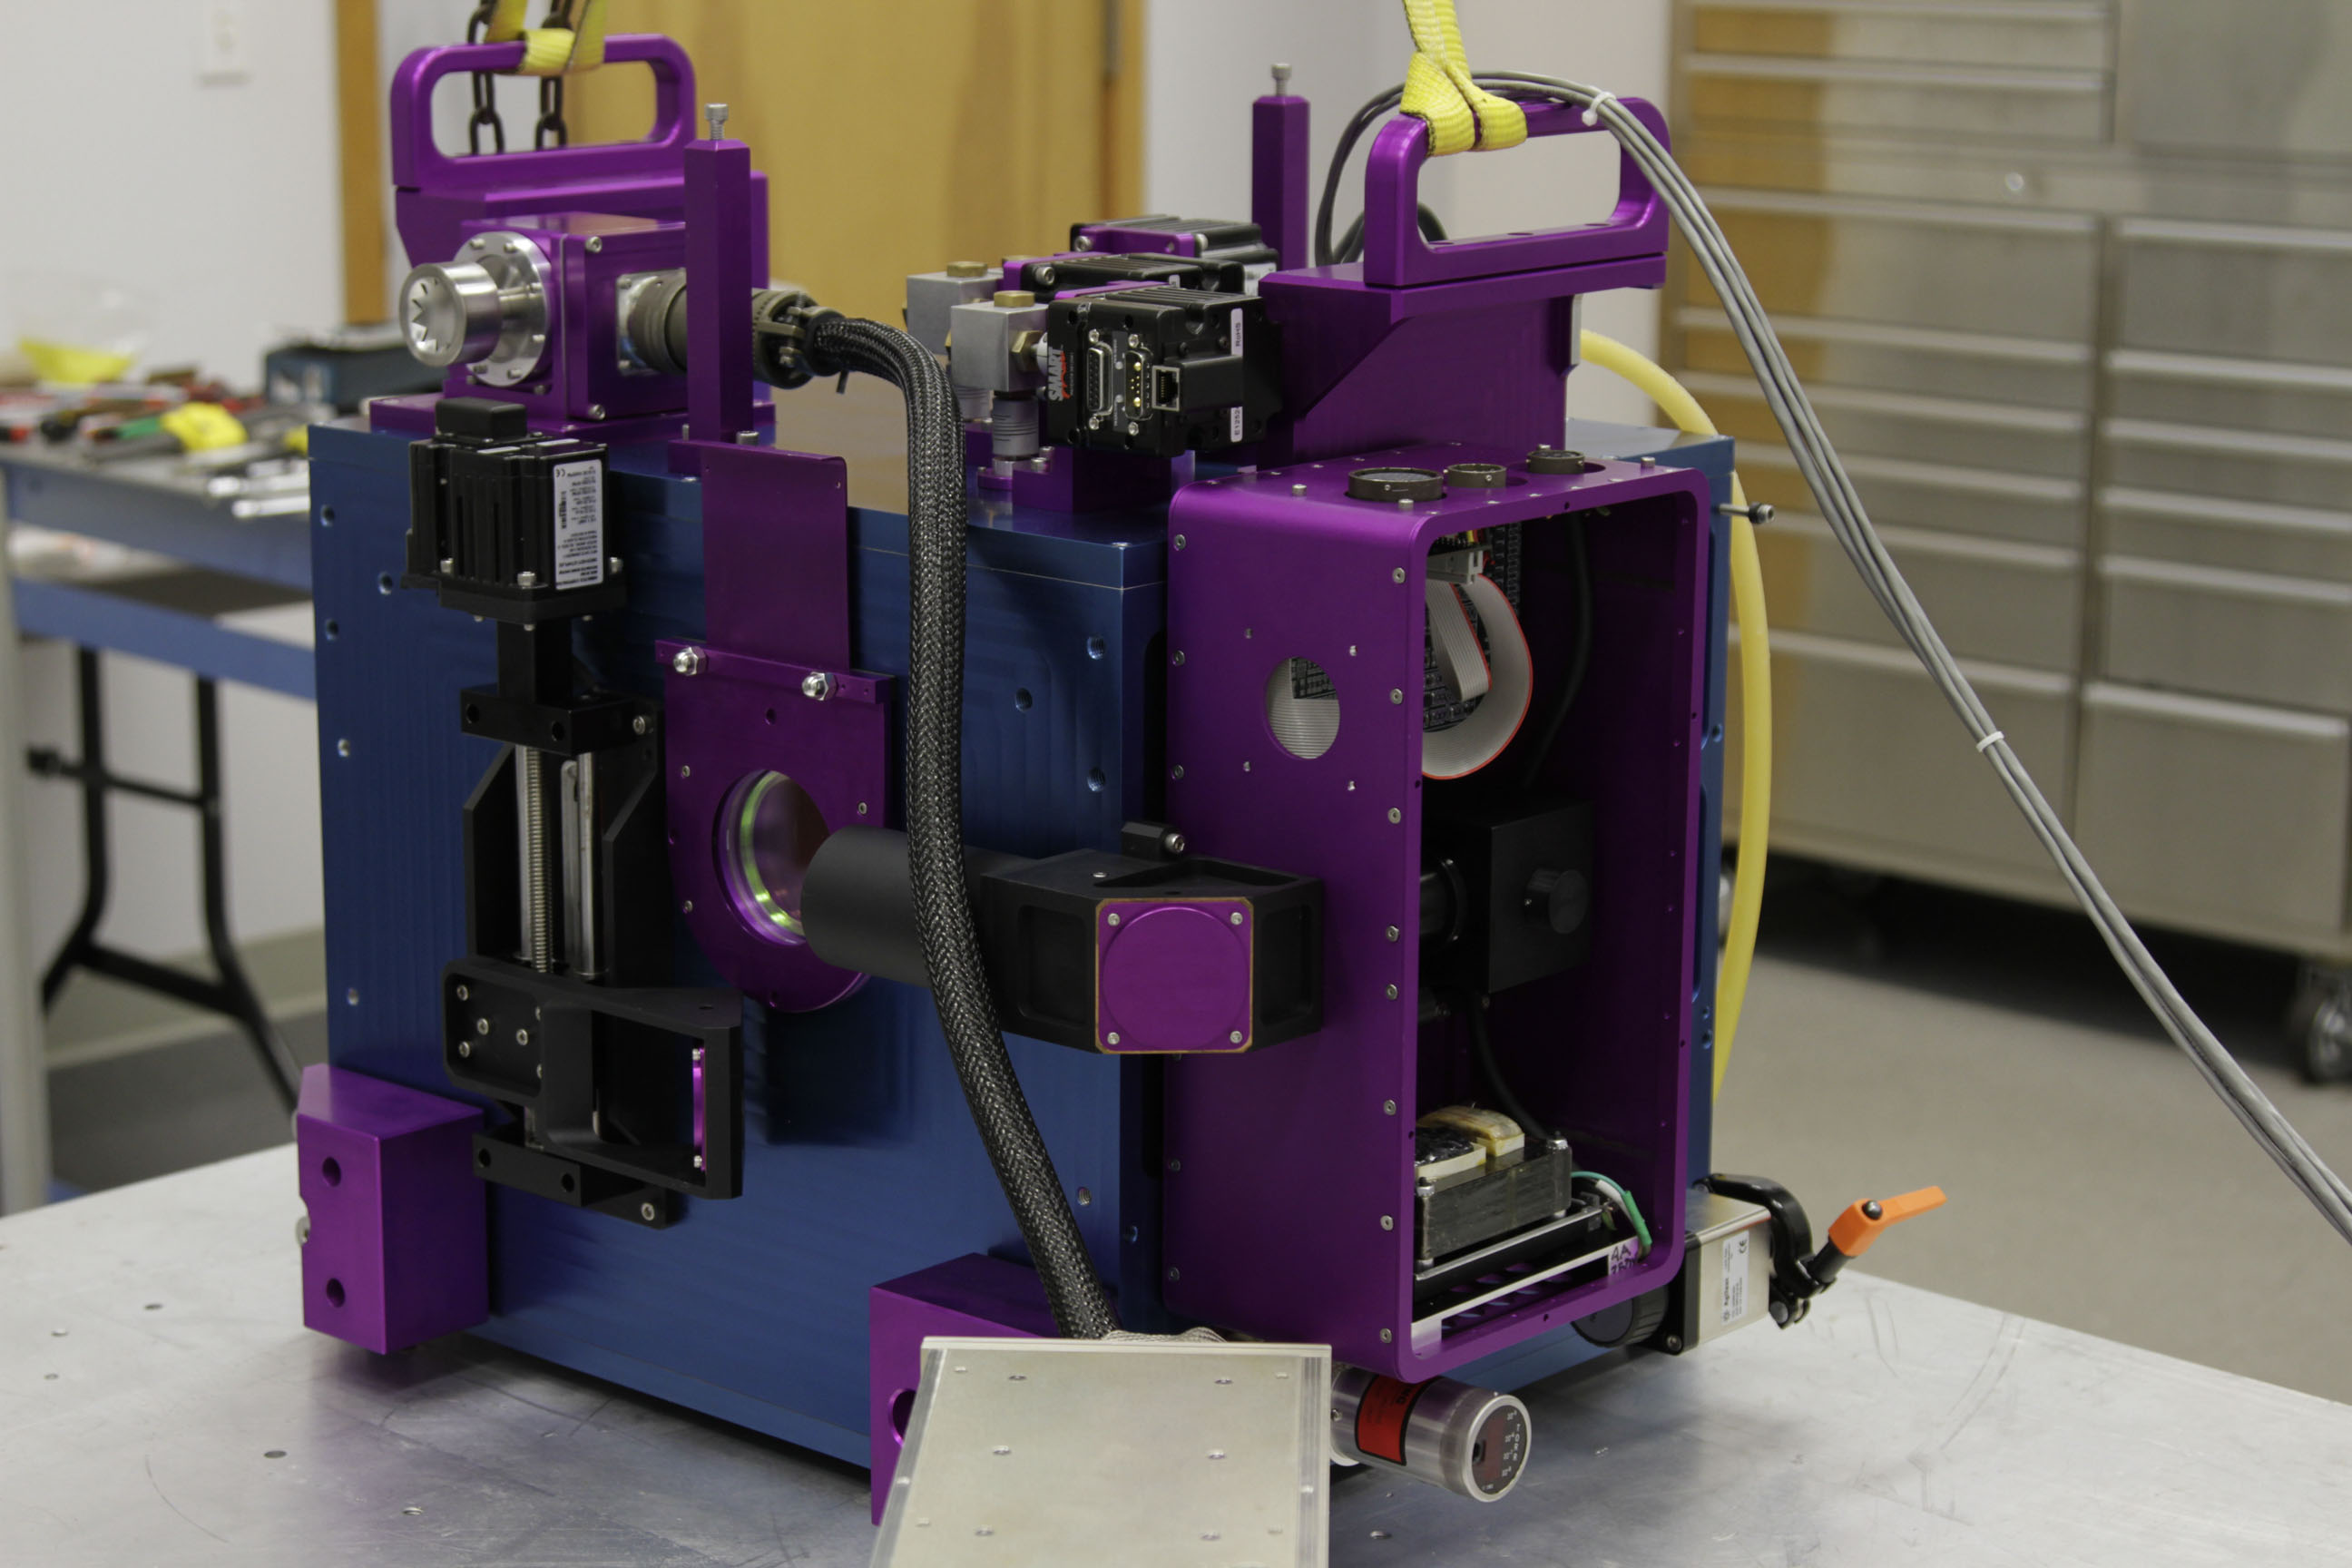
\includegraphics[width=\linewidth]{11}
\caption{Внешний вид устройства ASTRONIRCAM.}
\label{fig:1}
\end{wrapfigure}
& &Основной задачей данной работы является определние эффективности инфракрасной камеры прибора ASTRONIRCAM при работоте в спетроскопическом режиме.

ASTRONIRCAM - это криогенно-охлаждае-мый щелевой спектрограф на спектральную область 1-2.5 мкм, установленный в фокусе Нэсмита\footnote{Система Нэсмита - это трехзеркальная модификация системы Кассегрена, в которой внутри трубы телескопа между главным и вторичным зеркалами установлено диагональное зеркало для отбрасывания изображения вбок. Таким образом, фокус телескопа, называемый фокусом Несмита, находится сбоку трубы. Такая оптическая схема позволяет нагружать телескоп громоздким наблюдательным оборудованием, без разбалансирования трубы.} 2.5-м телескопа Кавказской горной обсерватории ГАИШ МГУ имени М.В. Ломоносова. При работе в спектроскопическом режиме прибор позволяет получать спектры протяжённых и точечных астрономических объектов с разрешающей силой $R = \dfrac{\lambda}{\delta\lambda}\leq 1200$.

Подробнее про принцип и особенности работы прибора ASTRONIRCAM можно прочесть в \cite{Sulsky1994}.

\hfill\break

\section{Наблюдения}
Одним из первых этапов выполнения задачи являлось получение спектров исследуемой звезды HIP85382 звёздного класса A0V. Наблюдения проводились с использованием последовательно двух щелей STIT6 и SLIT7 и фотометрических фильтров: Y, J, H и K. Результаты наблюдений представлены на Рис. 2, Рис. 3 и Рис 4.
\begin{figure}[h]
\begin{minipage}[h]{0.50\linewidth}
\center{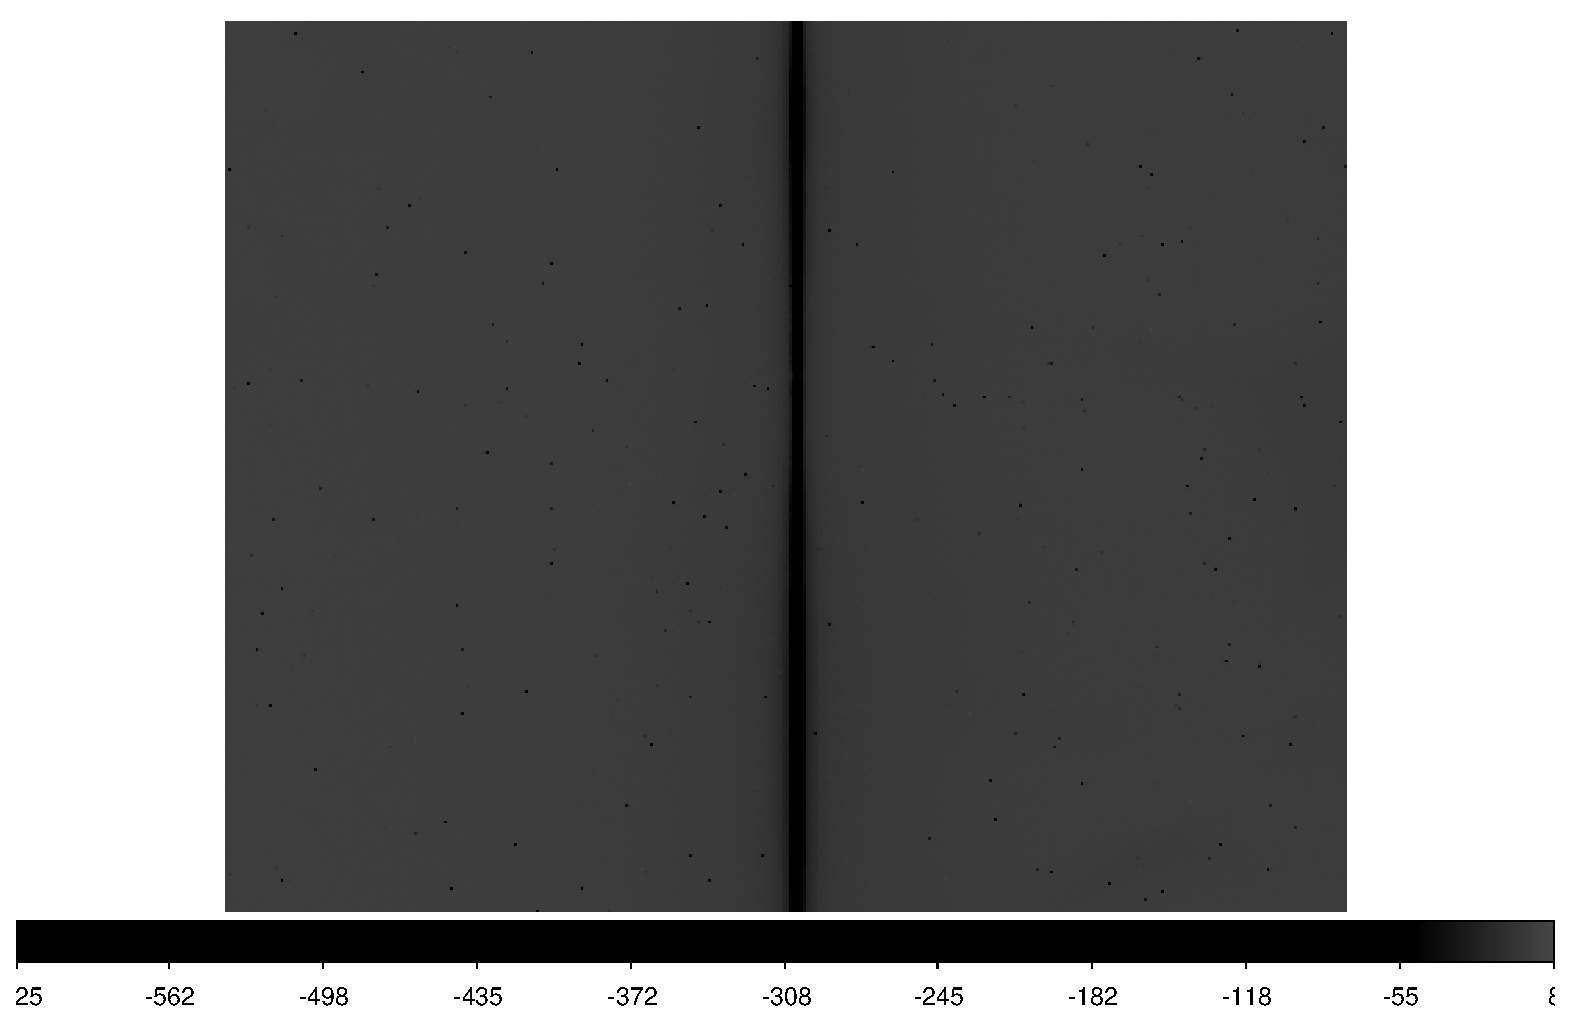
\includegraphics[width=0.75\linewidth]{SLIT6_Y} \\ фильтр Y}
\end{minipage}
\begin{minipage}[h]{0.50\linewidth}
\center{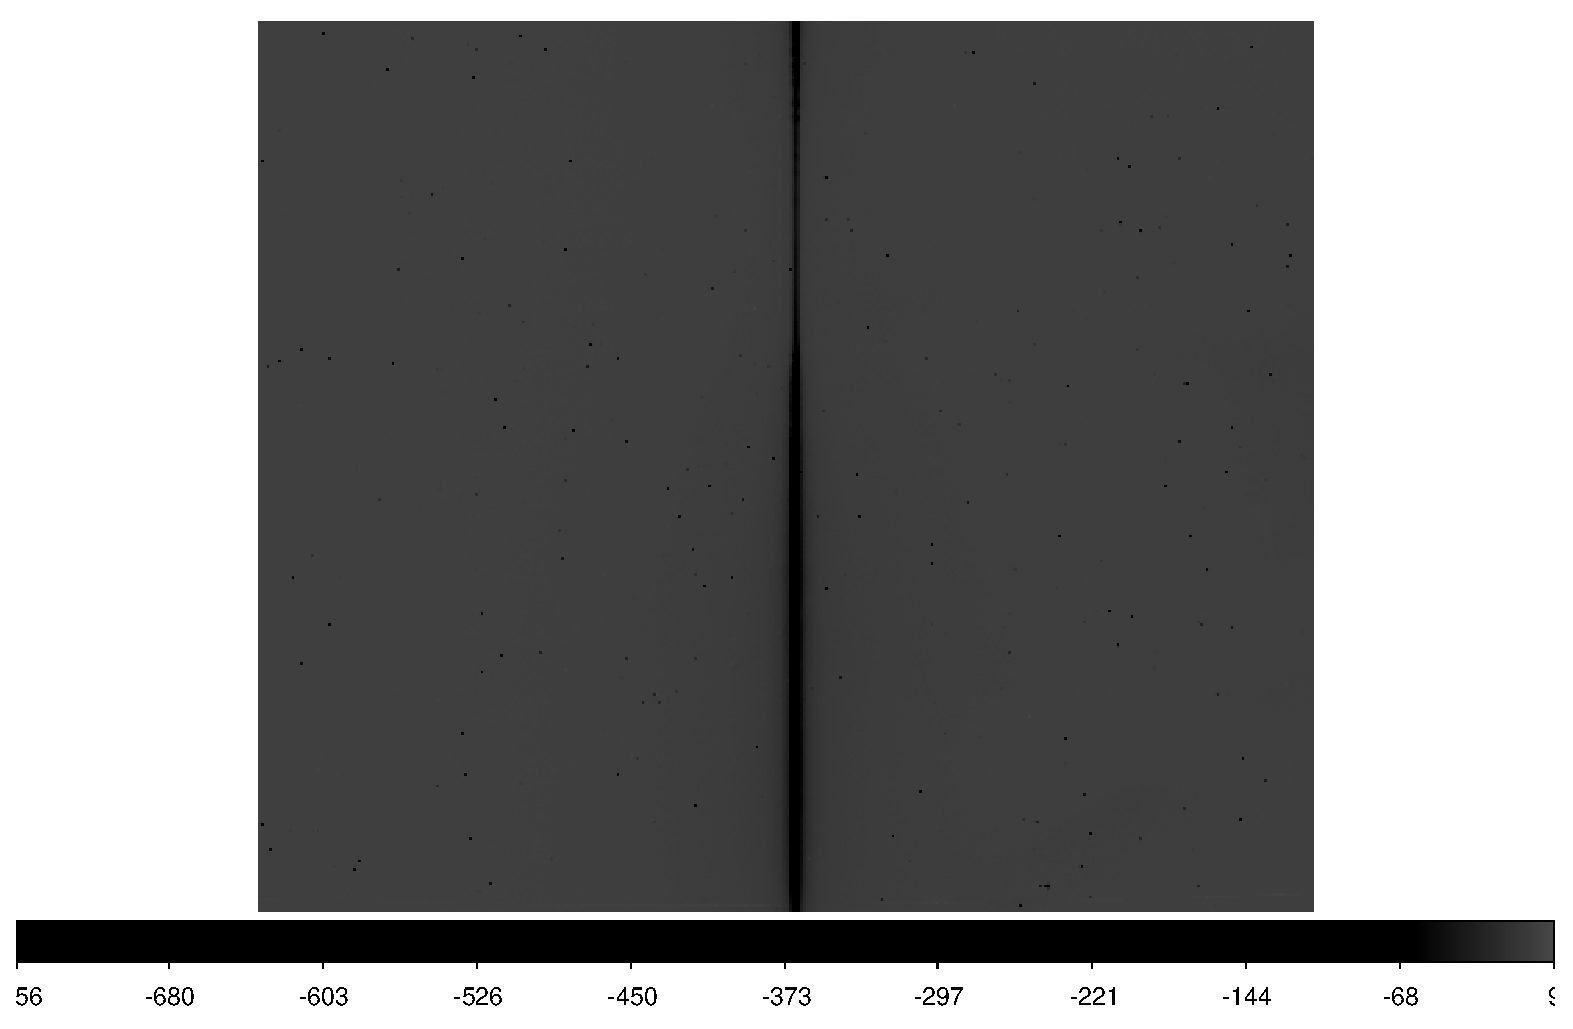
\includegraphics[width=0.75\linewidth]{SLIT6_J} \\ фильтр J}
\end{minipage}
\begin{minipage}[h]{0.50\linewidth}
\center{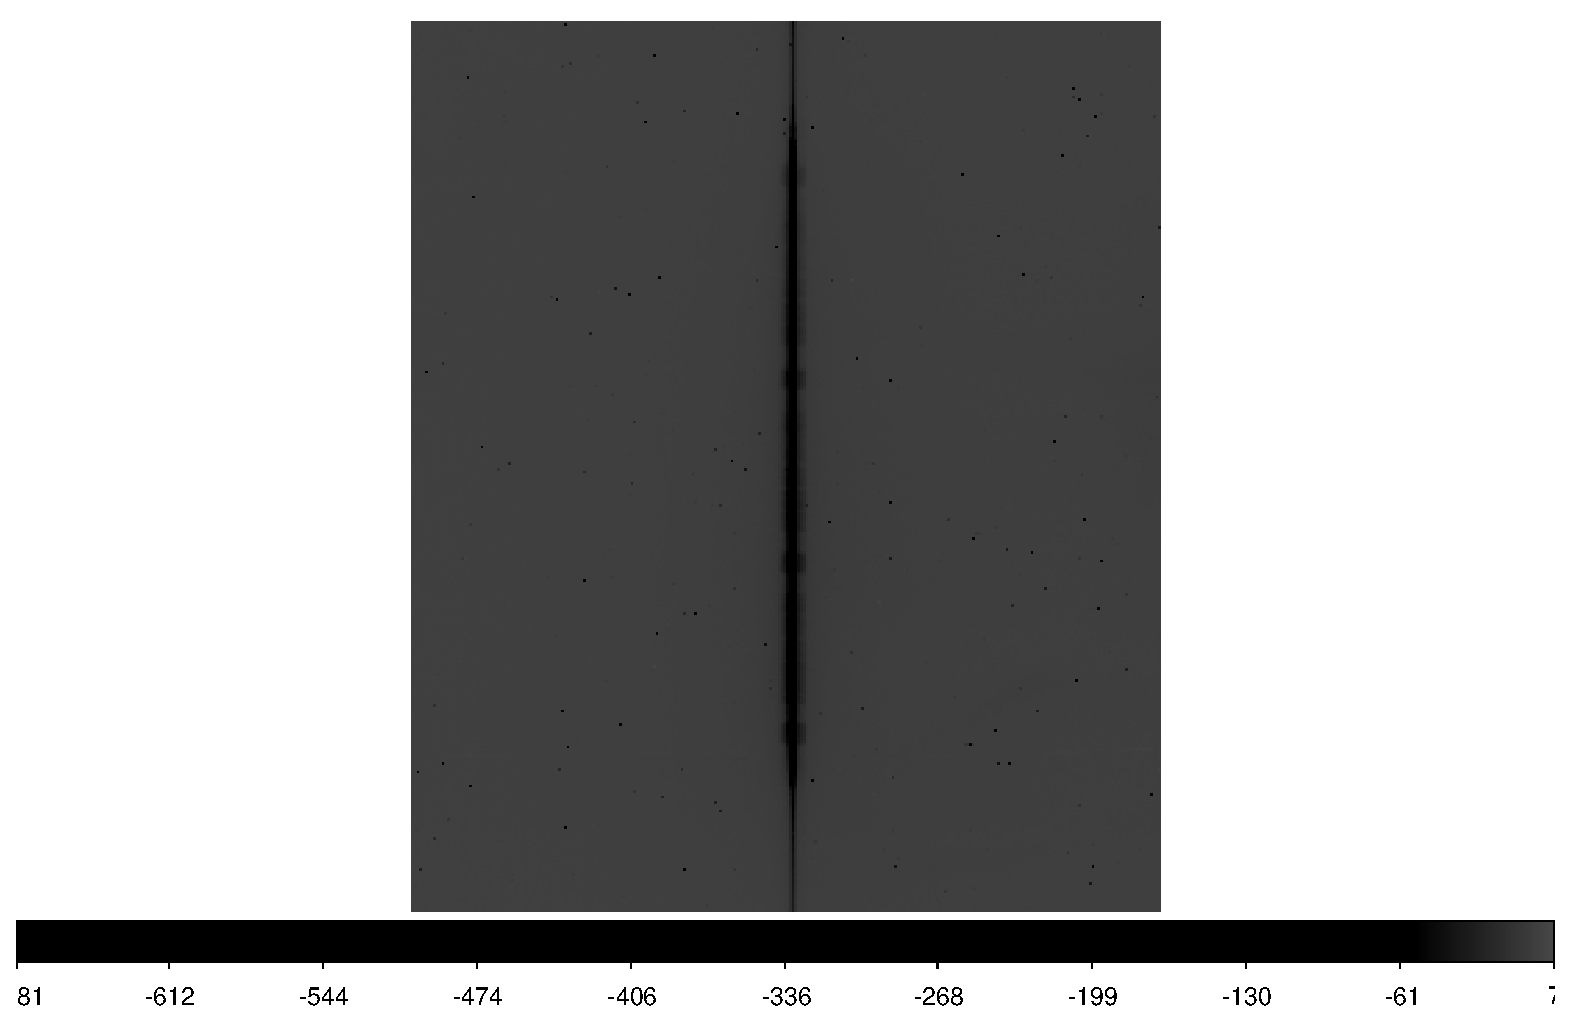
\includegraphics[width=0.75\linewidth]{SLIT6_H} \\ фильтр H}
\end{minipage}
\begin{minipage}[h]{0.50\linewidth}
\center{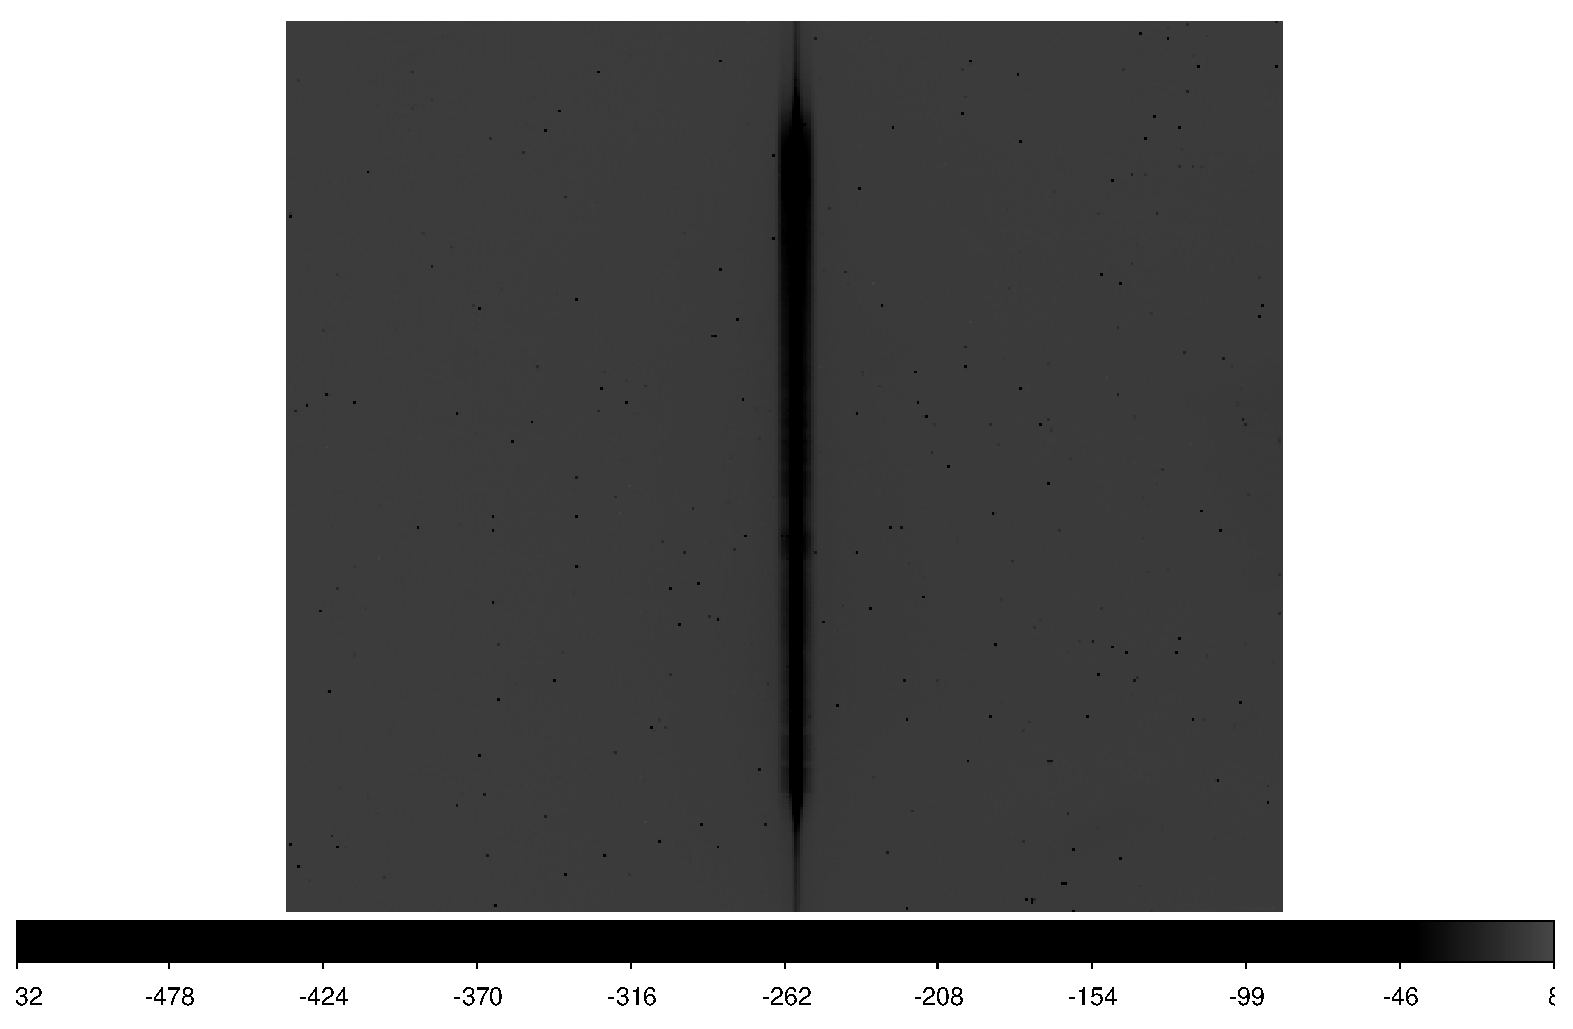
\includegraphics[width=0.75\linewidth]{SLIT6_K} \\ фильтр K}
\end{minipage}
\caption{Спектры звезды с использованием спектральной щели SLIT6.}
\label{ris:image1}
\end{figure}
\hfill\break
\begin{figure}[h]
\begin{minipage}[h]{0.50\linewidth}
\center{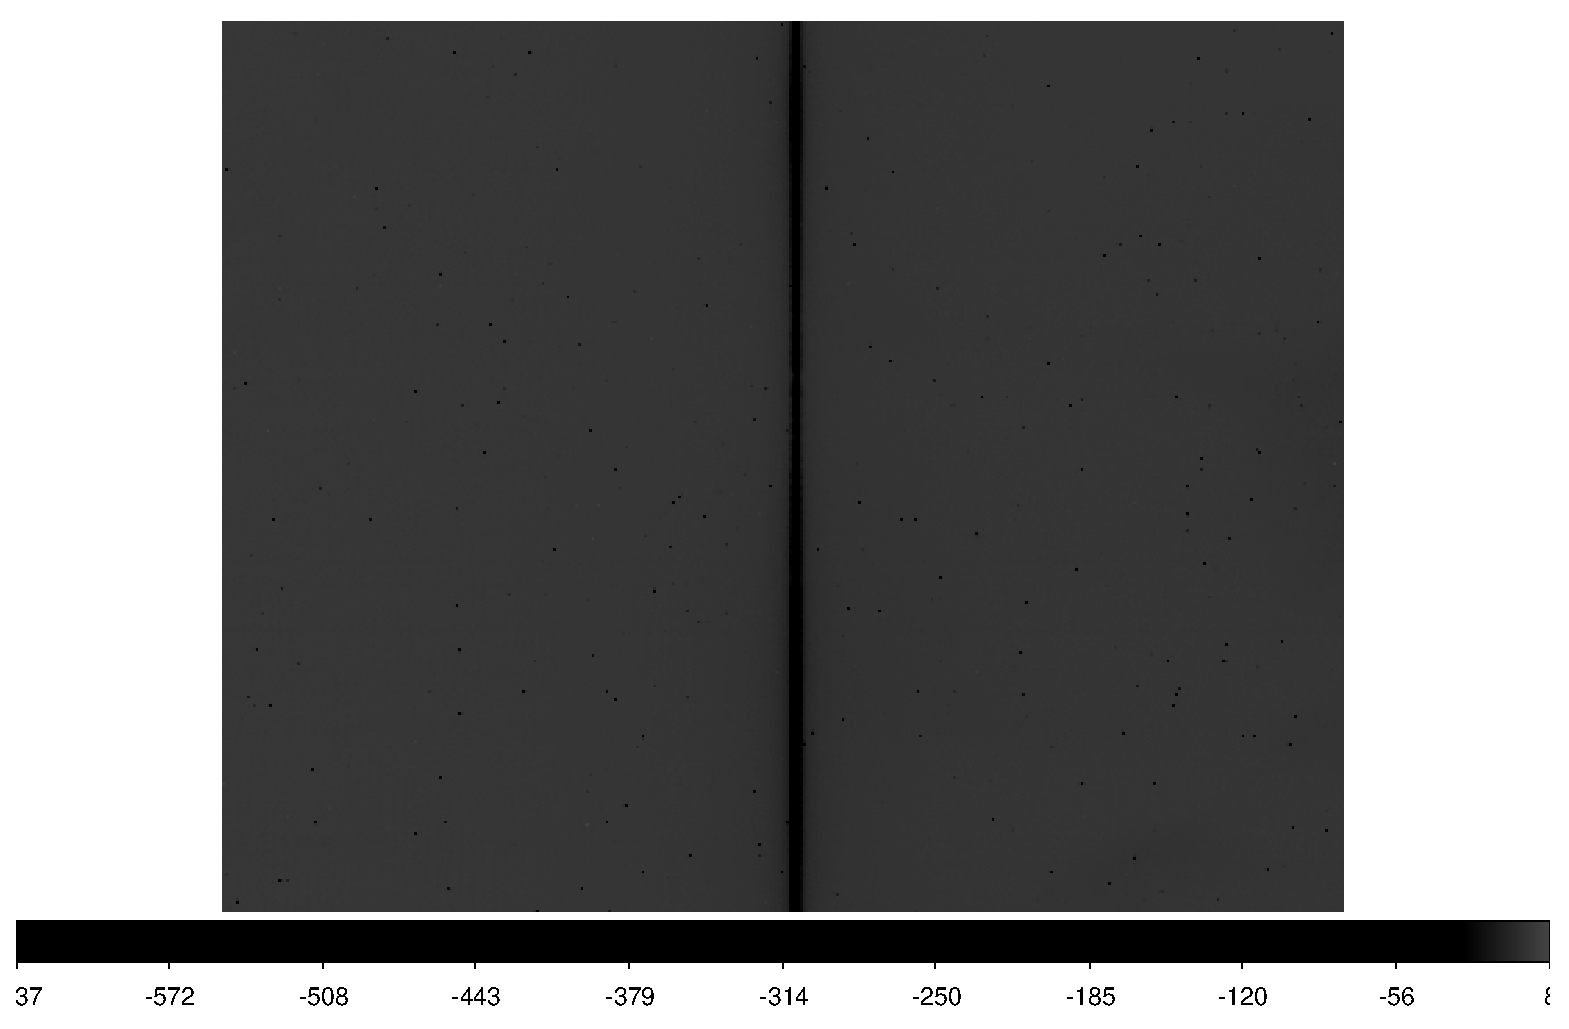
\includegraphics[width=0.645\linewidth]{SLIT7_Y} \\ фильтр Y}
\end{minipage}
\begin{minipage}[h]{0.50\linewidth}
\center{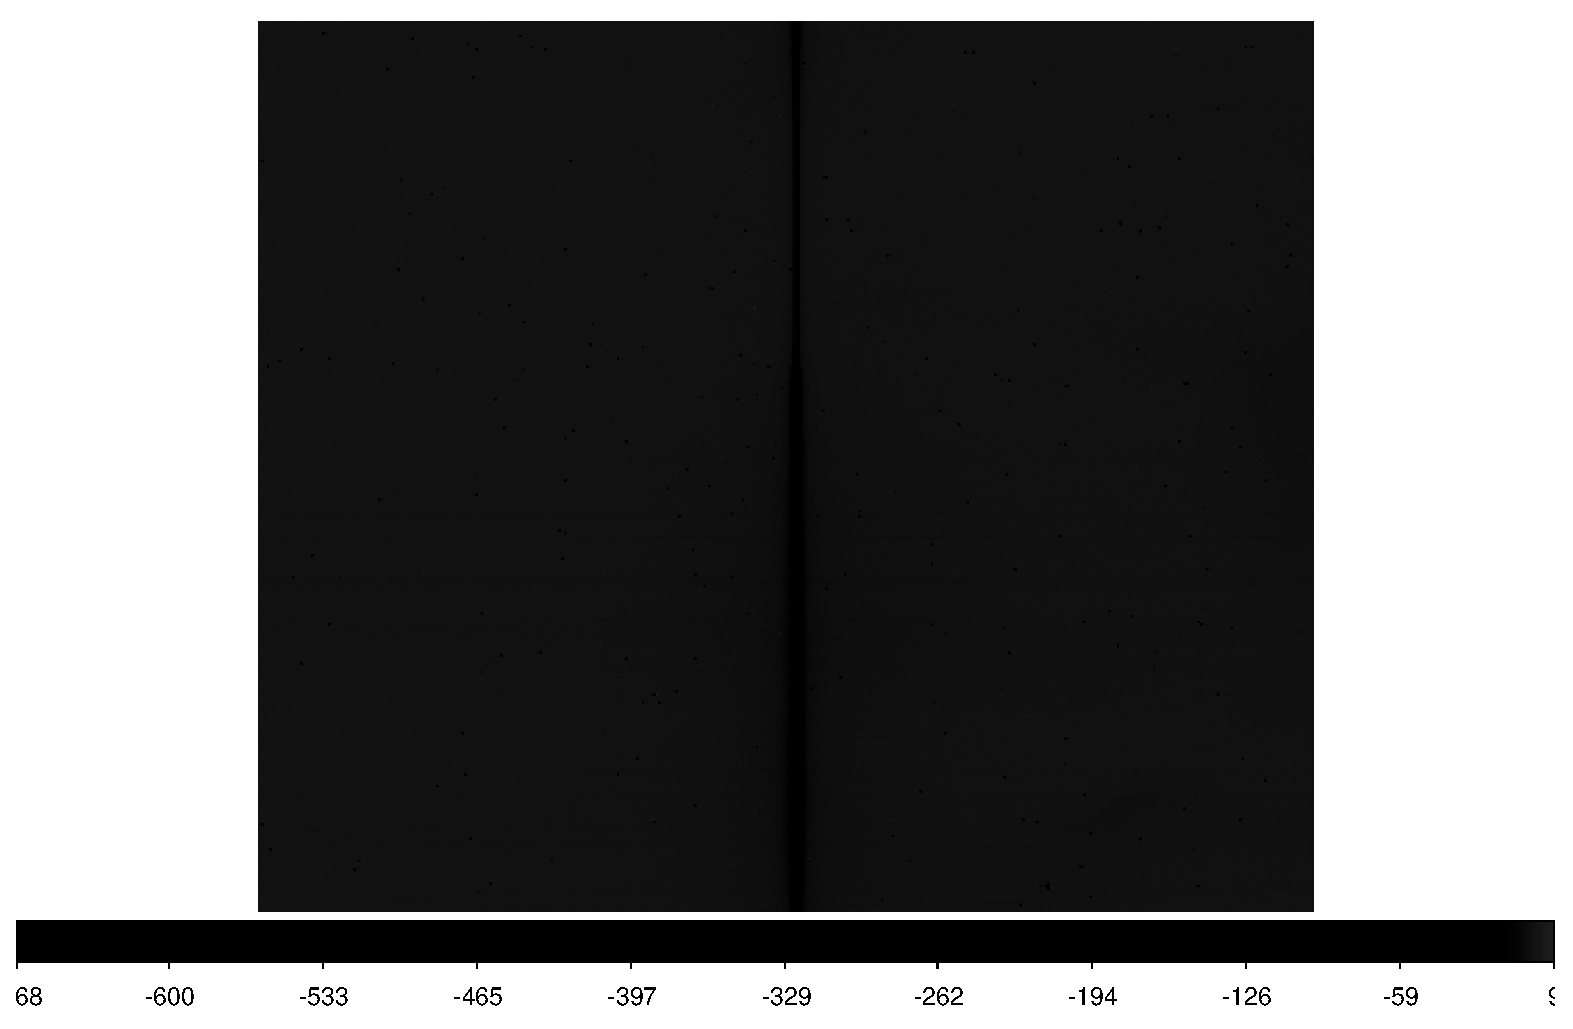
\includegraphics[width=0.64\linewidth]{SLIT7_J} \\ фильтр J}
\end{minipage}
\begin{minipage}[h]{0.50\linewidth}
\center{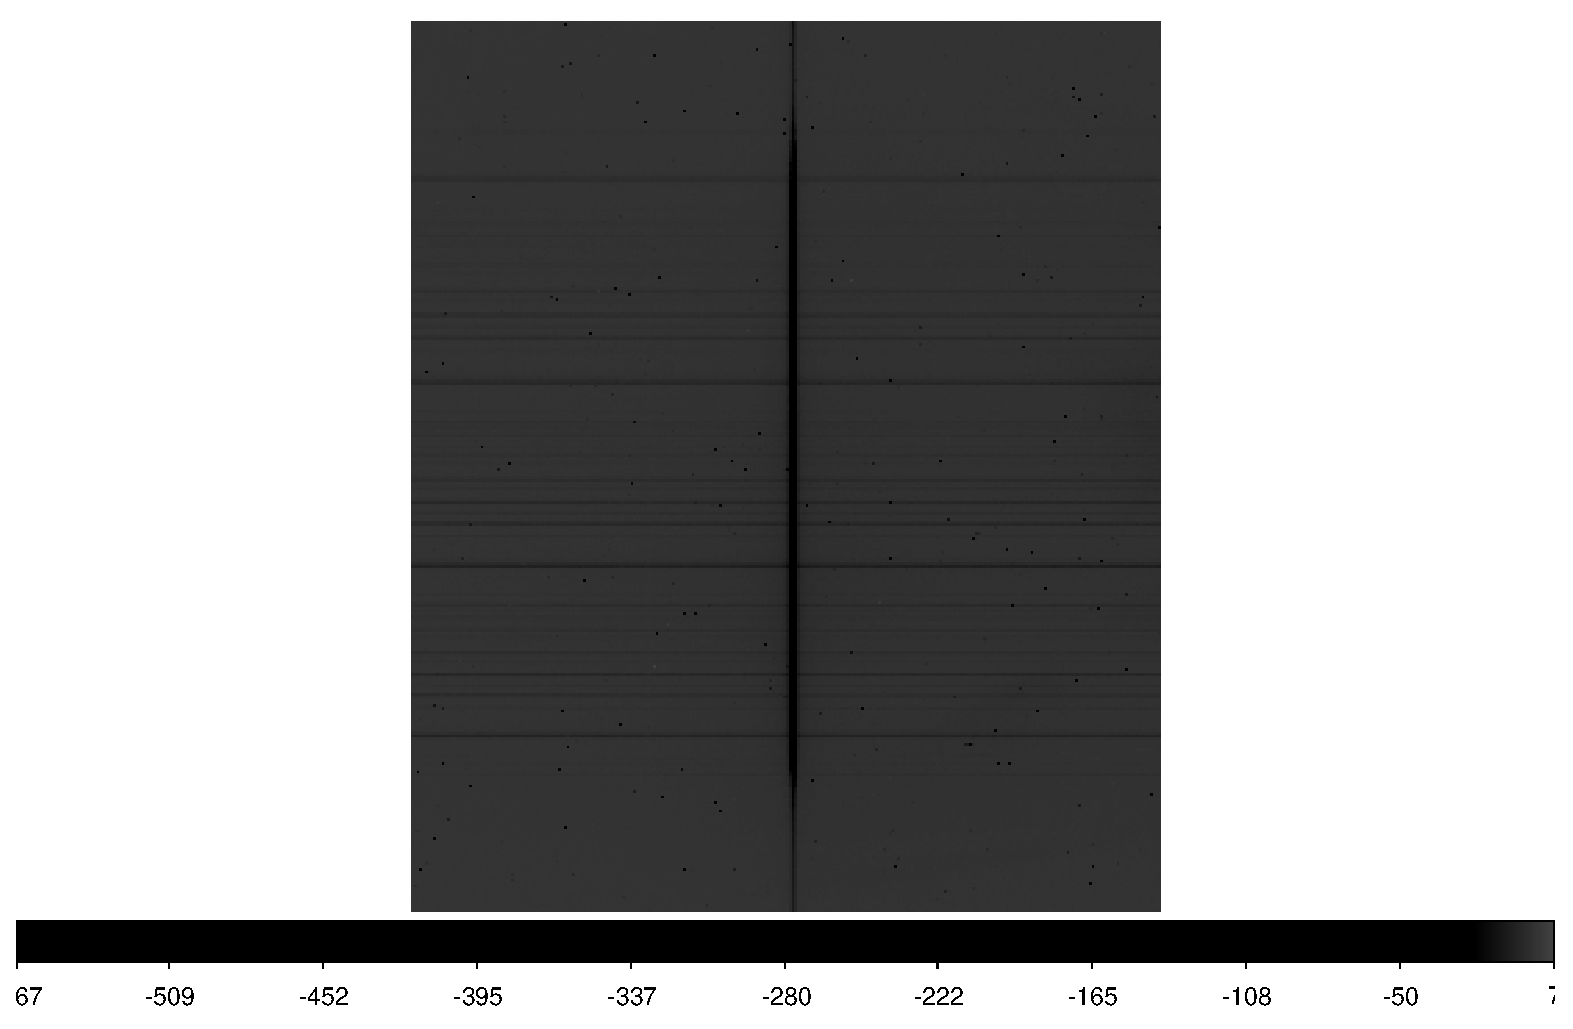
\includegraphics[width=0.64\linewidth]{SLIT7_H} \\ фильтр H}
\end{minipage}
\begin{minipage}[h]{0.50\linewidth}
\center{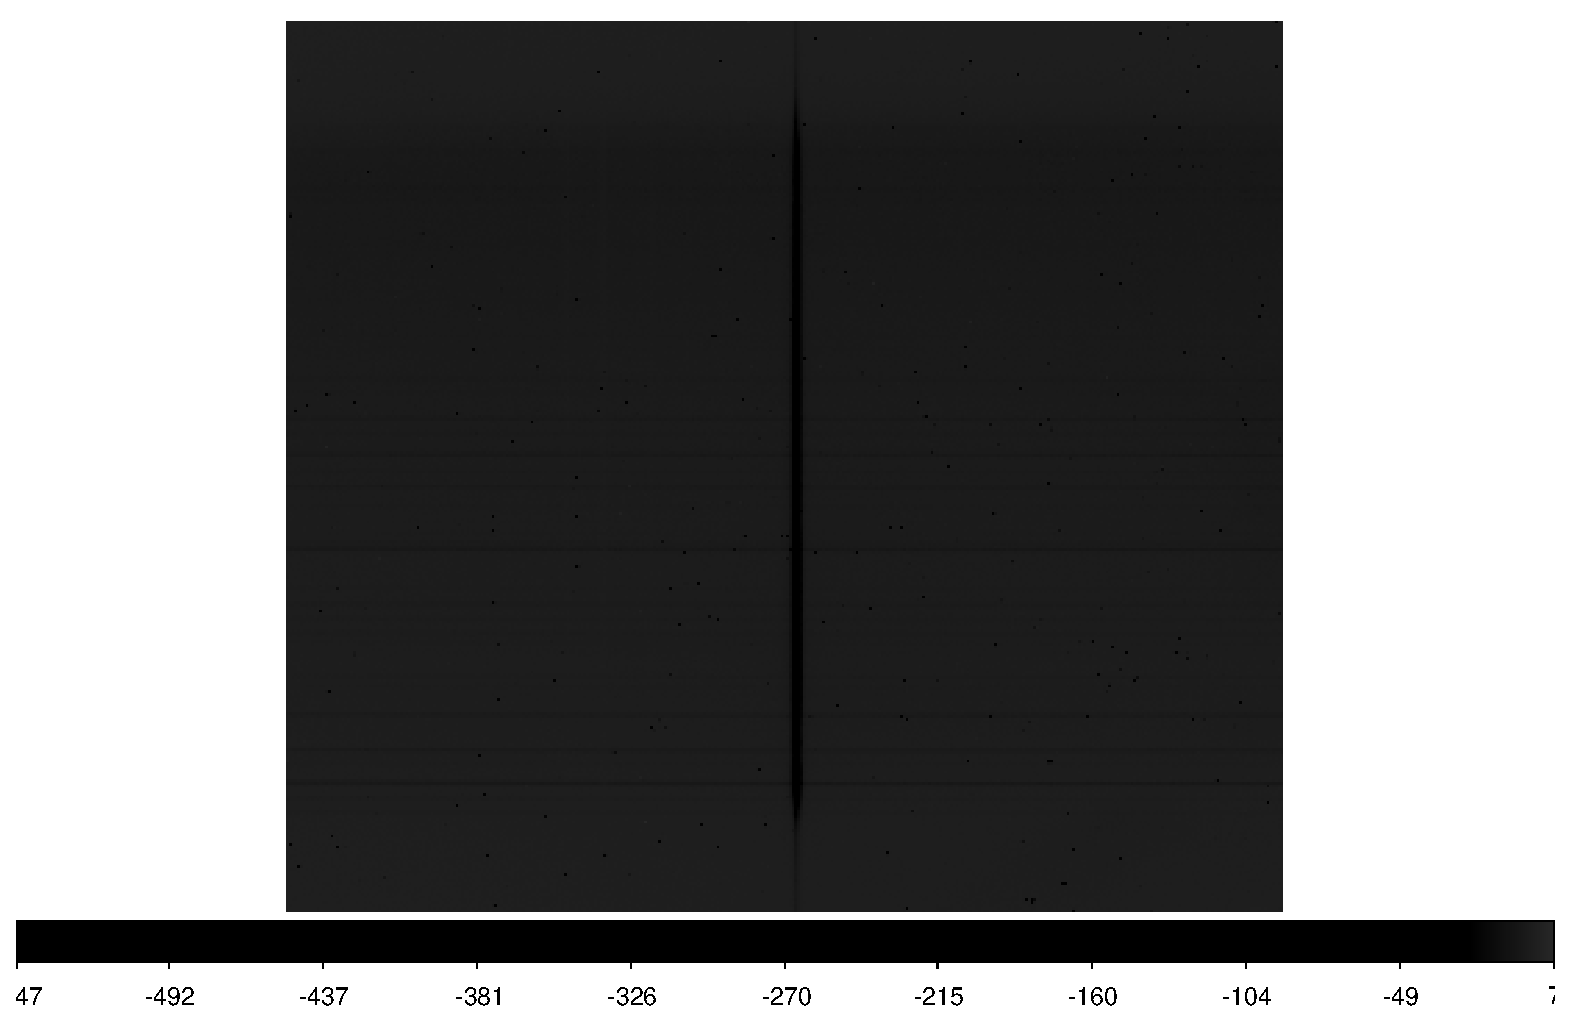
\includegraphics[width=0.64\linewidth]{SLIT7_K} \\ фильтр K}
\end{minipage}
\caption{Спектры звезды с использованием спектральной щели SLIT7 (с атмосферными полосами).}
\label{ris:image2}
\end{figure}

\begin{figure}[h]
\begin{minipage}[h]{0.50\linewidth}
\center{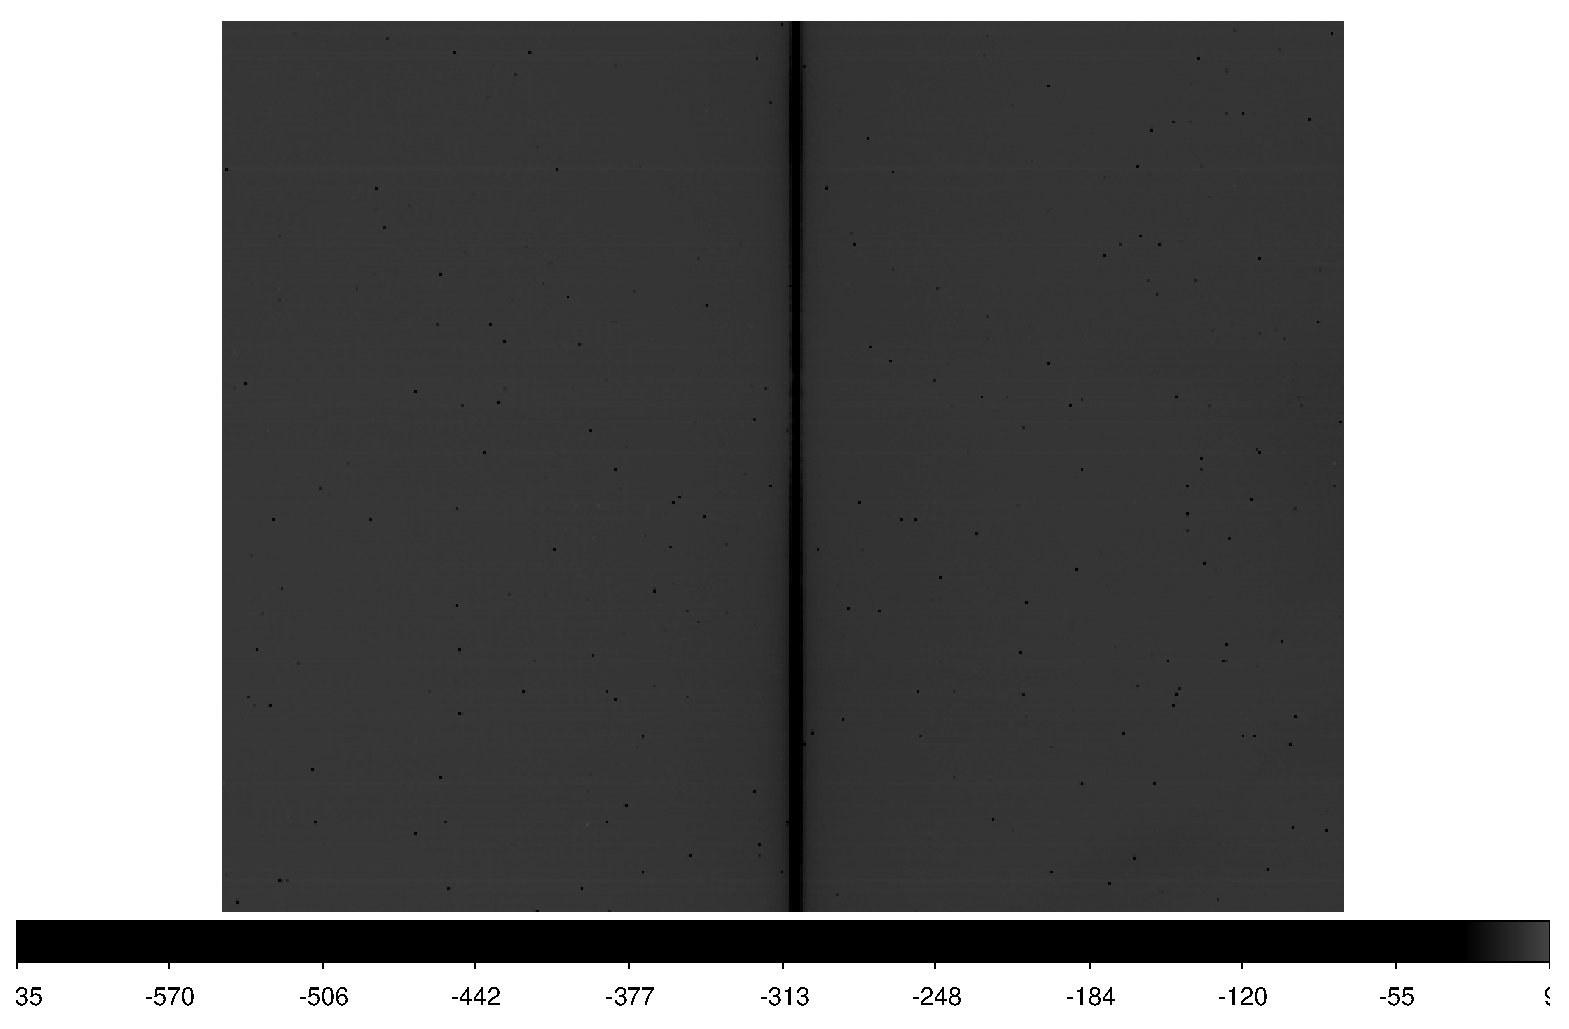
\includegraphics[width=0.64\linewidth]{SLIT7_Yw} \\ фильтр Y}
\end{minipage}
\begin{minipage}[h]{0.50\linewidth}
\center{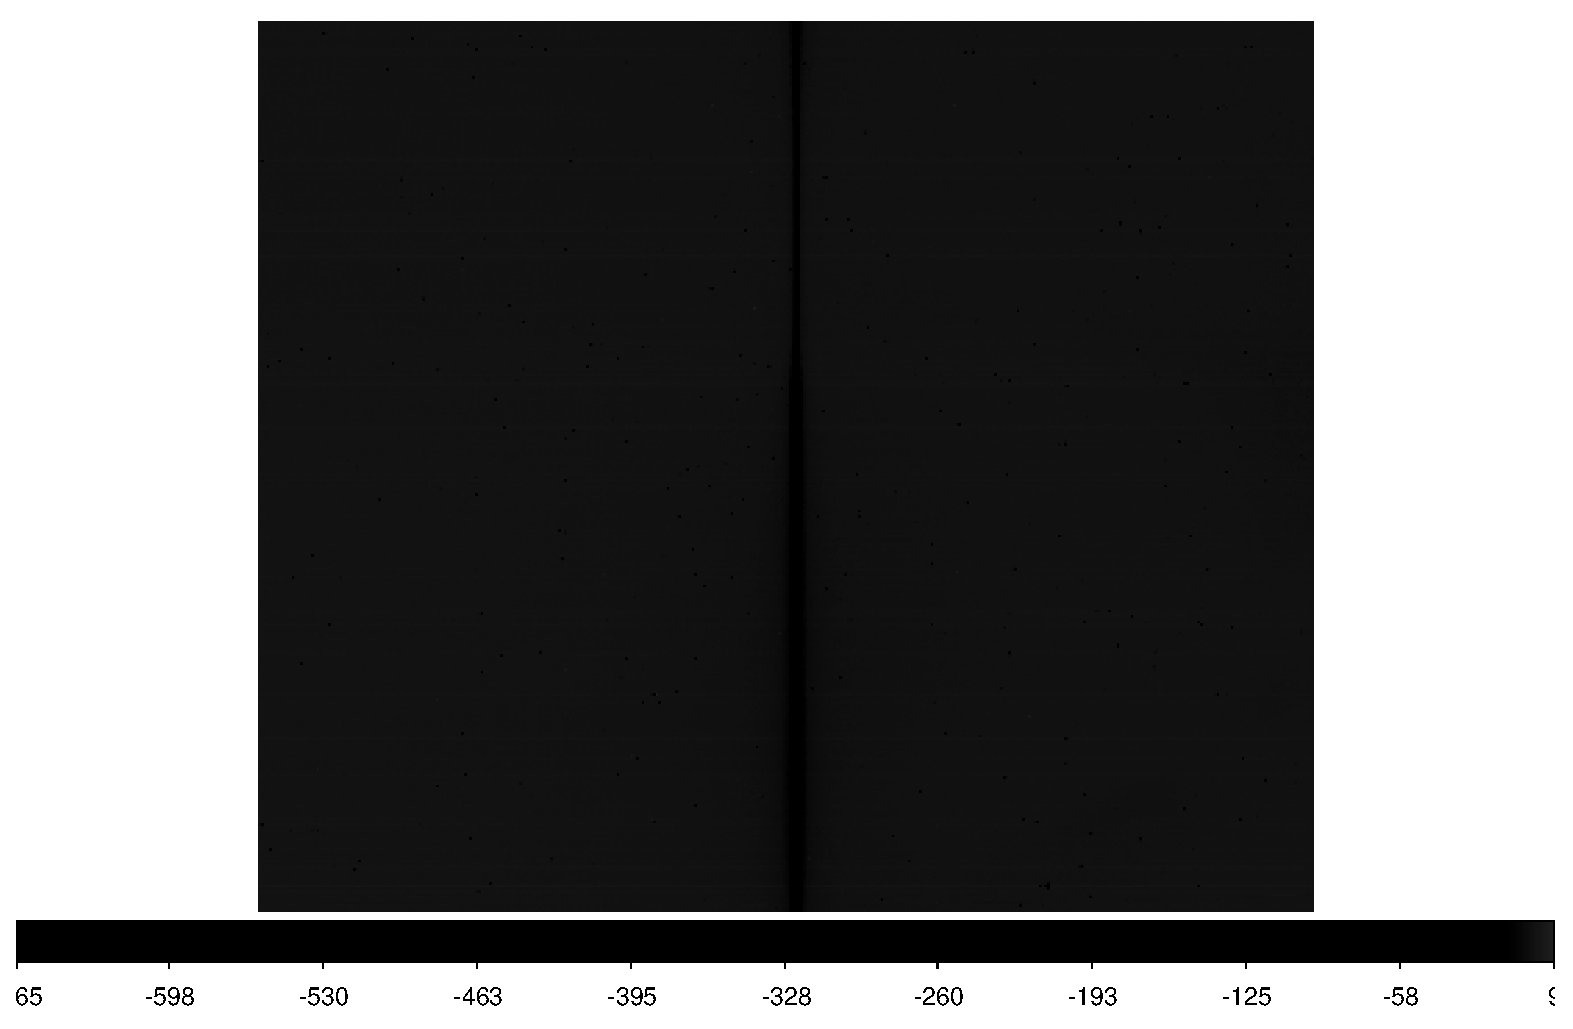
\includegraphics[width=0.64\linewidth]{SLIT7_Jw} \\ фильтр J}
\end{minipage}
\begin{minipage}[h]{0.50\linewidth}
\center{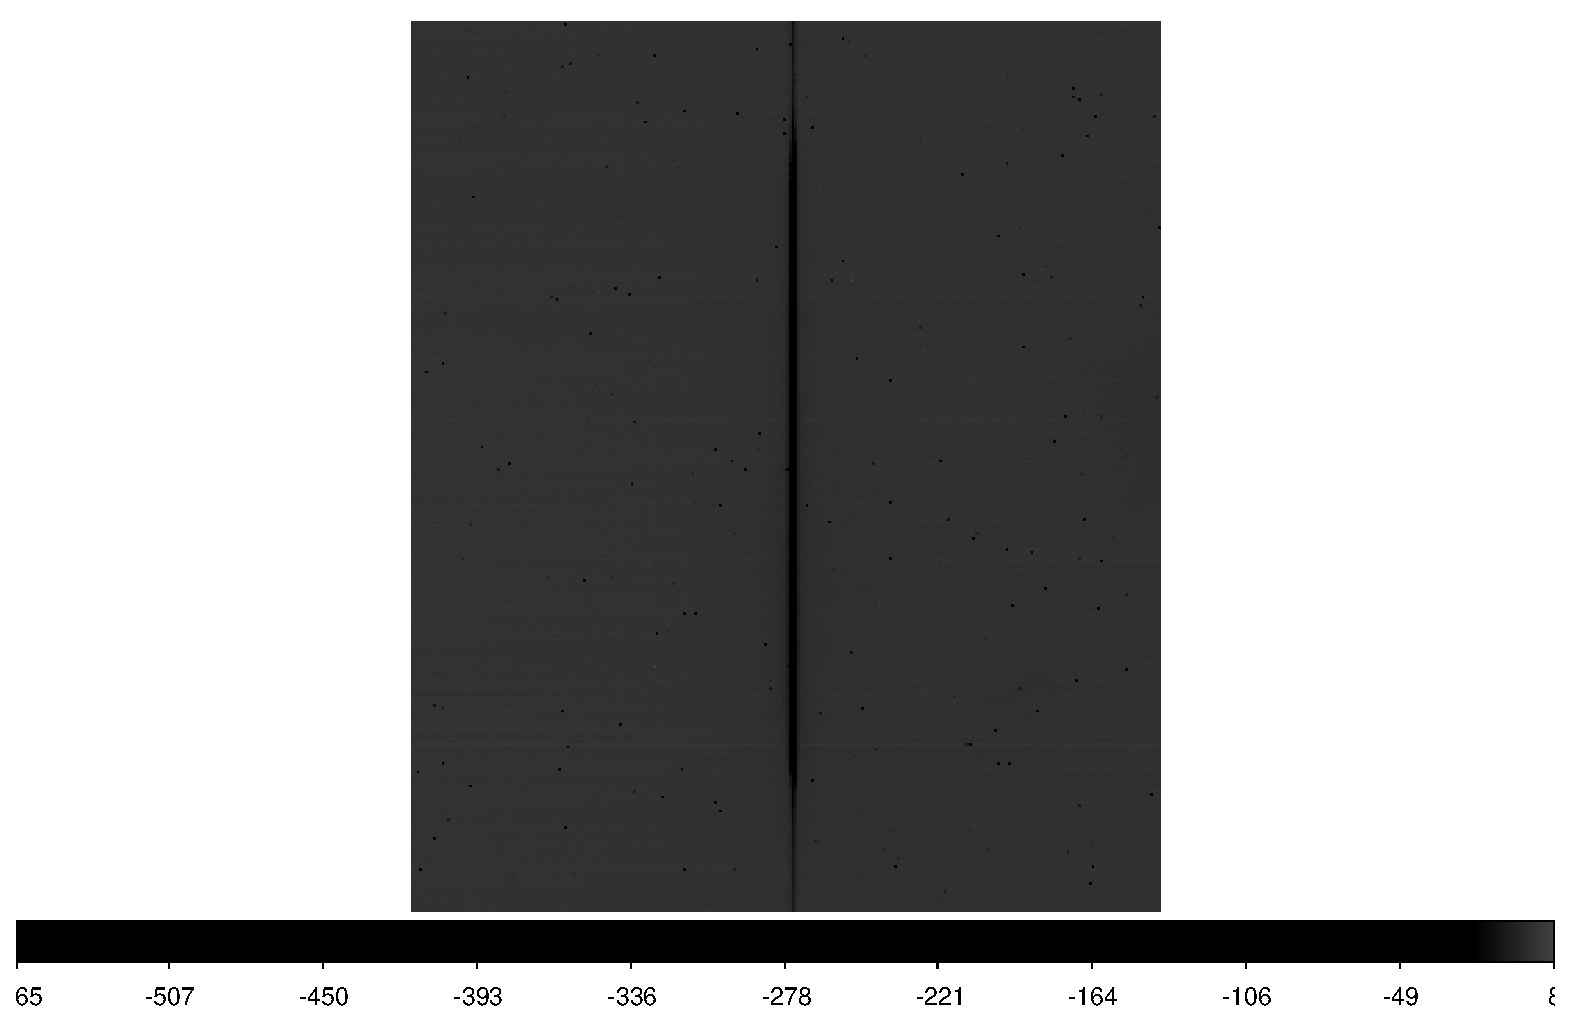
\includegraphics[width=0.64\linewidth]{SLIT7_Hw} \\ фильтр H}
\end{minipage}
\begin{minipage}[h]{0.50\linewidth}
\center{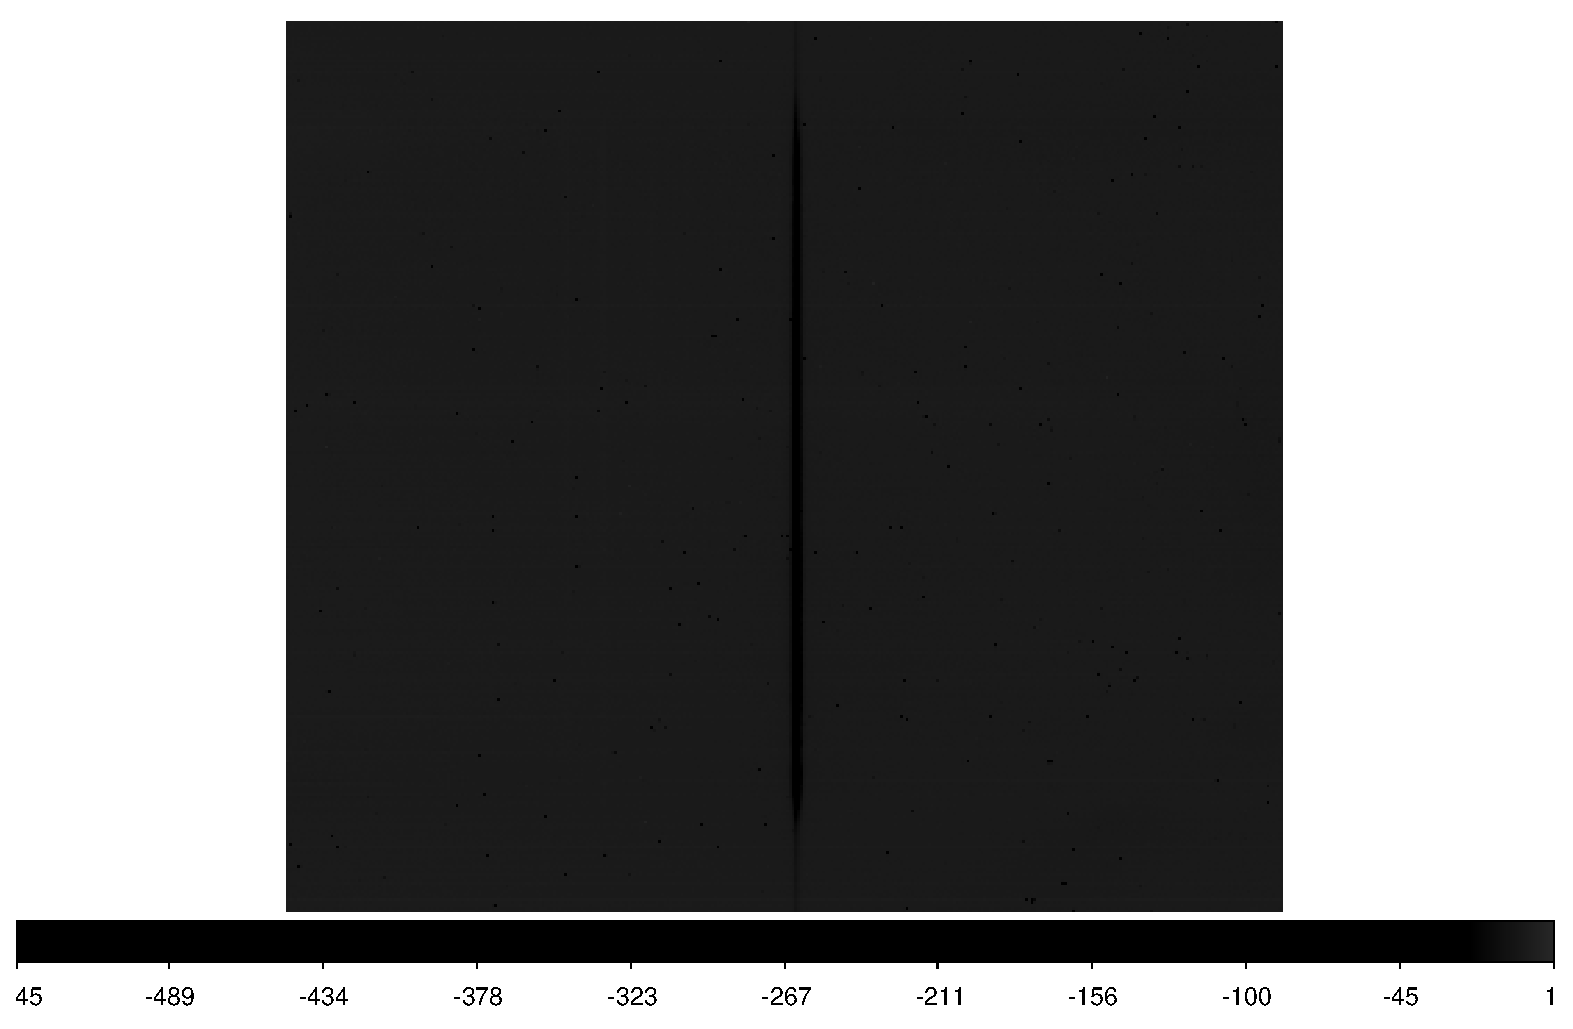
\includegraphics[width=0.64\linewidth]{SLIT7_Kw} \\ фильтр K}
\end{minipage}
\caption{Спектры звезды с использованием спектральной щели SLIT7 (без атмосферных полос).}
\label{ris:image3}
\end{figure}

В дальнейшем, с помощью обработки данных спектров была определена эффктивность инфракрасной камеры при использовании спектральных щелей SLIT6 и SLIT7.

\hfill\break

\section{Обработка данных}







\hfill\break

\section{Заключение}
В результате проделанных наблюдений, по результатам которых были получены спектры звезды HIP85382 звёздного класса A0V с использованием фотометрических фильтров Y, J, H и K, для спектральных щелей SLIT6 и SLIT7 и последующей обработки этих спектров были получена величины эффективности инфракрасной камеры прибора ASTRONIRCAM при использовании спектральных щелей SLIT6 и SLIT7, как процентная величина отношения общего числа фотонов, зарегистрированных детектором прибора за всё время экспозиции, к общему числу фотонов, которые достигли границы атмосферы за всё время экспозиции. Влияние атмосферы не учитывалось, так как оно невелико. В результате было получено, что величины пропускания камеры при использовании спектральной щели SLIT6 и различных фильтров следующие:     .Также, было получено, что величины пропускания камеры при использовании спектральной щели SLIT7 и различных фильтров следующие:          . Из полученных значений можно сделать вывод, что пропускание спектральной щели SLIT6 больше, чем пропускание спектральной щели SLIT7.

\hfill\break

\begin{thebibliography}{3}
\bibitem{Sulsky1994}
А. Э. Наджип, А. М. Татарников, Д. У. Туми, Н. И. Шатский, А. М. Черепащук, С. А. Ламзин, А. А. Белинский,  ASTRONIRCAM - инфракрасная камера-спектрограф 2.5-м телескопа КГО ГАИШ, (16 июня 2017 г.).
\end{thebibliography}
\end{document}


\end{document}  % КОНЕЦ ДОКУМЕНТА !